\documentclass[oneside]{book}

%TODOTODOTODOTODOTODOTODOTODOTODOTODOTODOTODOTODOTODOTODOTODOTODOTODOTODO
%juiste git commit voorzien!!!

% Load the VUB package.
% This has many options, please read the documentation at
% https://gitlab.com/rubdos/texlive-vub
\usepackage{vub}

%href package to make references clickable.
\usepackage{hyperref}
\hypersetup{
    colorlinks,
    citecolor=black,
    filecolor=black,
    linkcolor=black,
    urlcolor=black
}

%subfigures
\usepackage{caption}
\usepackage{subcaption}
\usepackage{wrapfig}

% Some highly suggested packages, please read their manuals.
\usepackage{cleveref}
\usepackage[natbib,style=apa]{biblatex}
\addbibresource{../bibliography.bib}

%space between paragraph and indent all
\setlength{\parskip}{1em}
\usepackage{indentfirst}

%space between bib entries
\setlength\bibitemsep{2\itemsep}

%images settings
\graphicspath{ {./images/} }
\usepackage{graphicx,caption}
\usepackage{float}
\usepackage{rotating}
\usepackage{tikz}

%fix section numbering for use with parts
\renewcommand*\thepart{\Roman{part}}
\makeatletter
\@addtoreset{section}{part}
\makeatother
\renewcommand*\thesection{\arabic{part}.\arabic{section}}
\renewcommand*\thesubsection{\thesection.\arabic{subsection}}

%START title
% done
\title{Animal classification AI}
\subtitle{Machine Learning}
\author{Lennert Bontinck}
\date{January, 2021}
\promotors{Master Computer Science: AI}
\faculty{Sciences and Bio-Engineering Sciences}
\begin{document}
\frontmatter
\maketitle
%END title


%START abstract
% done
\chapter*{Abstract}

This report documents the development of an \textit{animal classification AI} using a more \textit{old-school approach} of Visual-Bag-of-Words models.
This AI is capable of differentiating 12 different animals.
These models, and thus the AI, are developed in Python-based Jupyter Notebooks accompanied by this document.
This animal classification AI was developed as a fulfilment of the Machine Learning course requirements and was used to compete in the organised Kaggle competition \citep{kaggle_competition}.

Part \ref{part:about_the_code} of this report discusses the accompanied code in general.
Section \ref{section:inc_files} explains which files are the most important. 
Section \ref{section:ideology_dev_code} describes the ideology used to created the code. 
To make testing multiple models easier, \textit{a template} for model exploration was created and is discussed in section \ref{section:typical_model_exploration}.

In part \ref{part:data_analysis}, the \textit{data analysis} part of this project is discussed.
Section \ref{section:DA_data_distribution} talks about the \textit{unbalanced data} distribution.
In the next section, section \ref{section:DA_deeper_look_data}, a deeper look is taken into the data and possible \textit{preprocessing} is discussed.
The last few sections of this part discuss how the \textit{feature extraction} is dealt with and what the numerical representation looks like.

The \textit{linear baseline model} is discussed in part \ref{part:linear_baseline}.
This model is a fine-tuned \textit{Logistic Regression model} from the SciKit Learn library.
This model is often used to compare other models with.
Only models that perform better then this baseline model should be considered.
This part discusses the parameters used and the road to finding those optimal parameters.

Afterwards \textit{Support vector Classifiers} (SVC) are explored.
Part \ref{part:svc} discusses non-linear SVC models with different kernels and finds the \textit{rbf kernel} to be the best from three tested kernels.
Part \ref{part:linear_svc} focuses on linear SVC models in a similar fashion and finds them to perform worse.
An ensemble approach is discussed in part \ref{part:gradien_boost}.
This approach makes use of Gradient Boosting which, while interesting, didn't perform well.

It is chosen to do the model analysis in a separate part, part \ref{part:model_anal}.
Afterwards, part \ref{part:final_model} goes over some other possible optimisations considering what is learned from all experiments thus far.
Some of these are implemented whilst others are just discussed in a theoretical manner.
This results in the final, best performing, model.
Afterwards, in part \ref{part:conclusion}, a short conclusion is given.

It is noted that the page count of this document doesn't represent its actual length due to clear part separation from the used template and large figures.
Content that isn't crucial or is a repetition of supplied information is discarded or given as an appendix.
%END abstract


%TOC
\tableofcontents
\mainmatter

%START about
\part{About the code}
\label{part:about_the_code}

%------------------------------------

\section{Files accompanied by this report}
\label{section:inc_files}
Since this report discusses the development of an AI, \textit{a lot of code} is discussed as well.
This code is not shown inside this document but is available on the GitHub repository \citep{github_project}.
All code is written in Python-based Jupyter Notebooks.

%------------------------------------


\section{Ideology of the developed code}
\label{section:ideology_dev_code}
The Jupyter Notebooks have many inline comments and markdown blocks to make reading the code easier.
If code is extensively discussed in this report, a reference to the corresponding section is made inside the code. 
Some of the gathered results come from time-consuming function calls.
These can take \textit{multiple hours} to complete.
To spare some time, these results are saved in a Pickle file so they can be loaded in without having to do the function call.
The Notebooks are written in a way that makes testing multiple models easy, paying extra attention to reusability. 

%------------------------------------

\section{A typical model exploration}
\label{section:typical_model_exploration}
The testing of a model consists of two main parts.
Firstly the input of the model has to be optimized.
Afterwards, the (hyper)parameters of the model itself can be optimized.
These steps are clearly visible with the discussed models in this report since they follow a form of \emph{template}.
This template makes testing new models rather easy.
After optimizing everything in a standalone fashion, it has to be checked that these newly optimized parameters do not influence previously optimized parameters.
The resulting model should perform better than the linear baseline model in order to be considered.
Whilst many abstractions were made and creating a \emph{one-call pipeline} is possible, it's chosen to not do so.
This is because \textit{human reasoning} can be required in finding truly optimal parameters.
It also makes understanding and discussing the model easier.
After all, the goal of this report is to gather an understanding on how these models work, not solely  to get the best Kaggle score.

%------------------------------------


\section{Technical remarks}
\label{section:technical_remarks}

Most source files, for this report and the created models, are available on GitHub \citep{github_project}. Some files, like the used training images, were not included in this GitHub repository. Details about this can be found on the GitHub page (\texttt{README} file). Rights to this GitHub repository can be asked from the author. This report was created in \LaTeX{} by modifying the VUB themed template from Ruben De Smet (\citeyear{latex_template}).

%START data analysis
\part{Data analysis}
\label{part:data_analysis}

%------------------------------------

\section{About this part}
\label{section:DA_about_part}
Before rigorously testing different models available, it's important to take a look at the data that is supplied. The supplied data consists of 2 main groups of images, labelled training images and unlabeled test images.
As per the requirements of the Kaggle competition, the test images should only be used for evaluating the model on the Kaggle page by submitting a CSV of the prediction results.
Thus the test images can't be used for creating the model in any shape or form.
This means that only the labelled training images can be used to create and validate the model in development.
To avoid altering the model to perform well on the supplied test data and not in general, only the training data will be analysed.
All code used for this part is available under the developed code folder on GitHub, in the Jupyter Notebook \emph{data\_analysis.ipynb}.
This part describes how data can be analysed with the given code.
This code can be easily changed to analyse other variations of the data, e.g. using another descriptor.

%------------------------------------

\section{Data distribution}
\label{section:DA_data_distribution}
The provided labeled training data consists of 12 different classes.
There is a total of 4042 labelled training images supplied, the distribution of which is shown in figure \ref{fig:1-data_analysis-labeled_data_distribution}.
As visible in this figure, the distribution between classes is not balanced.
This has to be taken into account when fitting a model since some models will show unwanted behaviour when fitted with unbalanced data.
Luckily many solutions exist to minify the impact of this unbalance.
This unbalance has to be kept in mind when using a split of the training set as a validation set as well.
This is because such split might lead to a test set where some classes have considerably fewer instances in the test set and thus the performance on those classes has less impact on the total score, which may be unwanted.


\begin{figure}[H]
    \centering
    \fbox{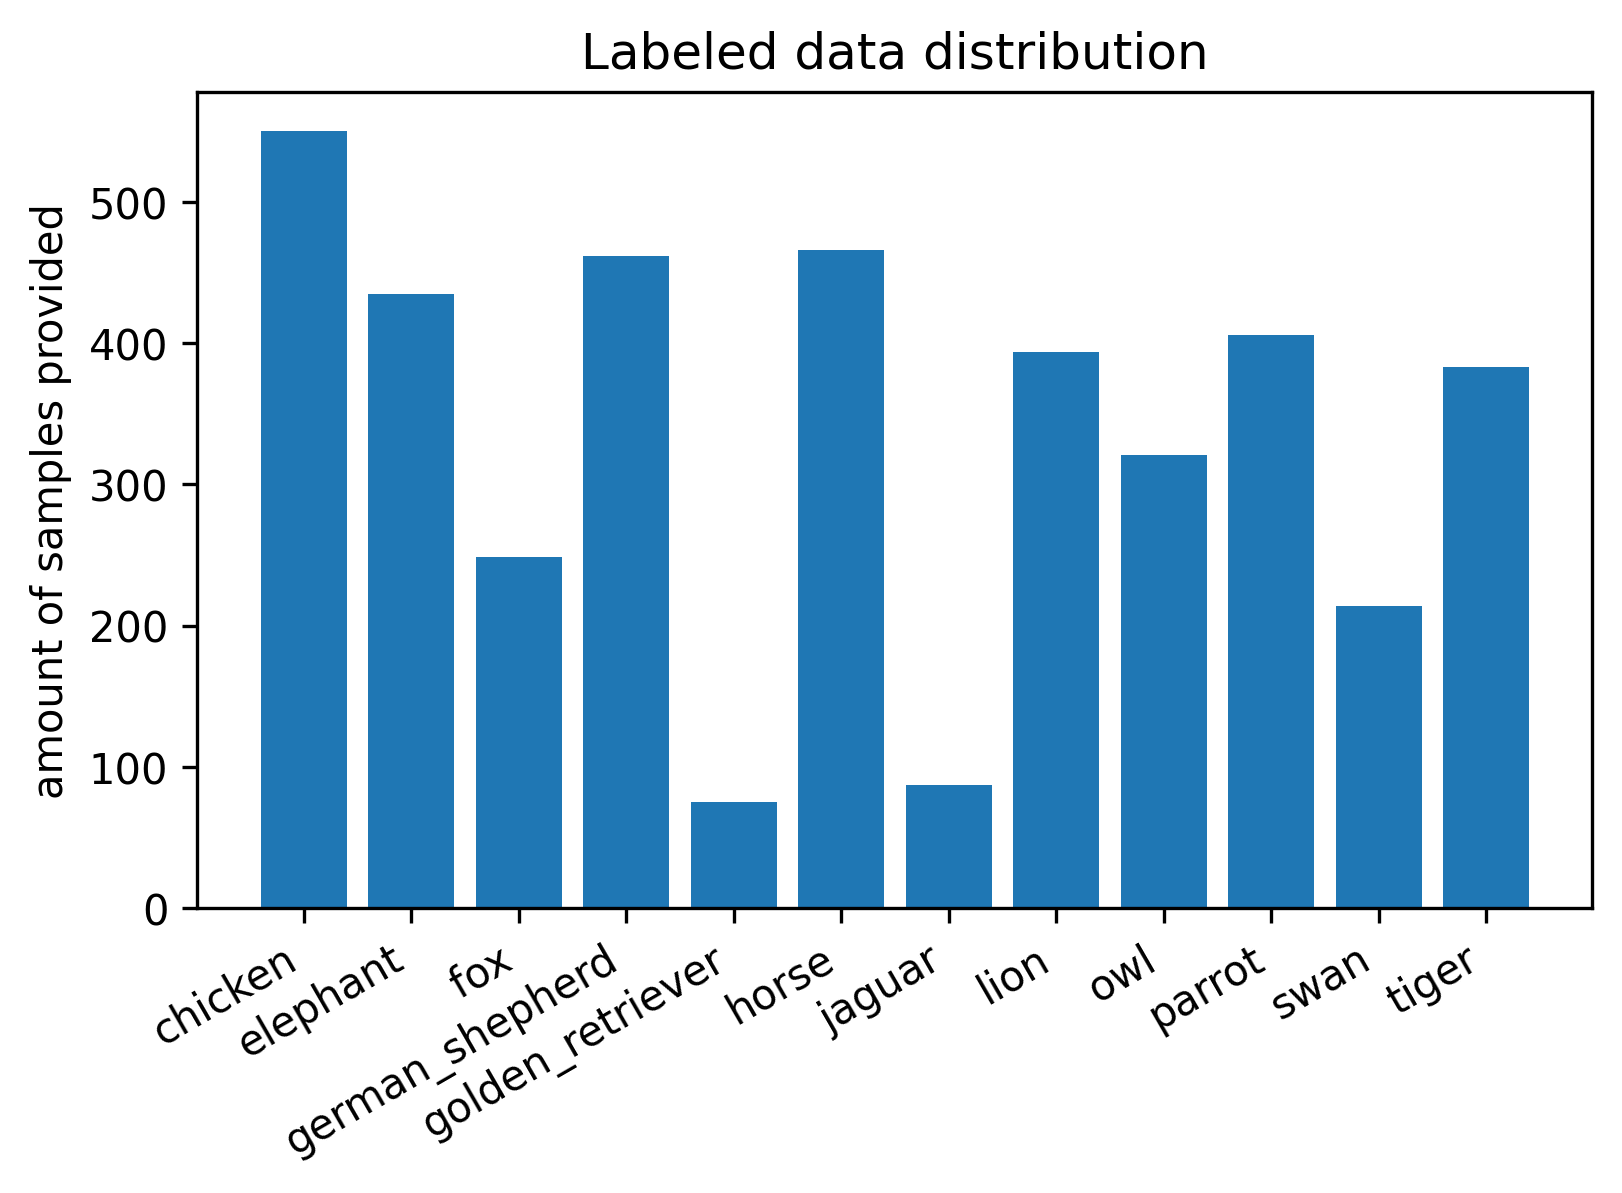
\includegraphics[width=0.7\linewidth]{images/1-data_analysis-labeled_data_distribution.png}}
    \captionsetup{width=0.65\linewidth}
    \captionsetup{justification=centering}
    \caption{The data distribution of the supplied training set.}
    \label{fig:1-data_analysis-labeled_data_distribution}
\end{figure}

%------------------------------------

\section{Deeper look at the training data}
\label{section:DA_deeper_look_data}

Whilst noting that the available data isn't balanced over all the classes is very important, there are also different aspects of the data that need analysing. 
An overview of the supplied training data is given in figure \ref{fig:1-data_analysis-labeled_data_overview.png}, available in the figures list at the end of this report.
This figure shows the first five images of each class.
From this, it becomes apparent that multiple factors of the data aren't \emph{optimal}.
This knowledge is important since it can aid in better prepossessing and in finding a better model in general.
The most noteworthy findings are listed here:
\begin{itemize}
    \item Images vary in shapes, some are taken in portrait, others in landscape.
    \item Images vary in size, some are high resolution whilst others are relatively low resolution.
    \item The framing of the subject(s) varies a lot. Sometimes the labelled animal is completely visible and centred in the frame. In some images there are multiple animals spread across the image, others show a close-up of the animal.
    \item Some images have a detailed background that makes up for a lot of the image, in others the background is blurry and its impact is presumably less.
    \item Some images have very vibrant colours in broad daylight, others are black and white in dimly lit environments.
\end{itemize}

This diversity in the provided training set is expected since it has been scraped from the web.
This also means that \emph{noise} can be expected, another important factor to keep in mind when choosing and optimizing models.
Many of the listed things can be minified by doing some clever prepossessing of the images.


%------------------------------------

\section{Feature extraction}
\label{section:DA_feature_extraction}

Since the focus of this competition is on developing great models and not necessarily on data prepossessing and feature extraction, some feature extraction has already been provided.
More info on the prepossessing and feature extraction provided is available in the provided notebook \emph{creating\_vbow.ipynb}.
In short, images are converted from there typical RGB representation to a numerical representation of interesting points, which can be used as input for our model.
How this is done will briefly be discussed here.

Instead of using the whole image as data, only a select few of \emph{interesting points} of the image are taken into consideration.
These interesting points of an image are found by using the \emph{Shi-Tomasi corner detector}.
The following important parameters for the \emph{features.extractShiTomasiCorners} function call are:
\begin{itemize}
    \item number of interesting points = 500
    \item minimum distance between interesting points = 20
\end{itemize}

Shown in figure \ref{fig:1-data_analysis-POI} is an example output of interesting points found by the Shi-Tomasi corner detector.
It's clear that this is far from optimal, but finding interesting points isn't an easy task and thus the results are better then they might seem on first sight.
This method might perform better after fine-tuning.

\begin{figure}[H]
    \centering
    \fbox{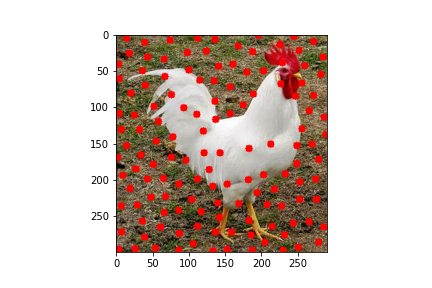
\includegraphics[width=0.8\linewidth]{images/1-data_analysis-POI.png}}
    \captionsetup{width=0.7\linewidth}
    \captionsetup{justification=centering}
    \caption{Example of points of interest found by Shi-Tomasi corner detector.}
    \label{fig:1-data_analysis-POI}
\end{figure}

Finding interesting points is only half of the work.
These interesting points now need to be represented by numerical values that have actual meaning, afterwards, they're clustered using a helper function.
Remember from section \ref{section:DA_deeper_look_data} that the provided images differ a lot.
Thus the numerical representation, generated by a descriptor, has to be so that it minifies the impact of different lighting, scaling...
The following descriptors are used and their outputs are provided: DAISY, ORB, FREAK, LUCID, VGG, BoostDesc, SIFT.
Whilst SURF is another great descriptor, it's not provided nor is the license available for this project.
SIFT is often referred to as the most famous and successful of these descriptors, but all of them should be explored.
Clustering is done by the \emph{createCodebook} function which uses Mini-Batch K-Means clustering from the SciKit Learn library.
This is also something that might be fine-tuned.

%------------------------------------

\section{The numerical representation}
\label{section:DA_numerical_representation}

As discussed in section \ref{section:DA_feature_extraction}, the images are stored as numerical representations using descriptors.
To save time, these numerical representations for all the descriptors are stored in a separate \emph{Pickle} file.
Since these representations form the input of a model, it's important to get a grip on how these look.
The provided \emph{createCodebook} function is used for clustering this data, which was also discussed in the previous section.
This function allows specifying how many clusters should be created for clustering the interesting points.
These different clusters can be thought of as different \emph{features}.
The function returns 2 lists.
The first contains the labels for the image represented at a certain index.
The other contains information about each image at that index.
This information is the output of the clustering done for that image and thus corresponds to an array which size equals the requested cluster amount.

An overview of the data from such clusters/features given by the SIFT descriptor is given in figure \ref{fig:1-data_analysis-labeled_data_overview.png}, available in the figures list at the end of this report.
From this, it is visible that the values seem to be normalized.
This would have to be checked for all descriptors used and perhaps some outliers would need to be removed.

In figure \ref{fig:1-data_analysis-correlation_matrix} the correlation matrix is shown for 30 clusters of the SIFT descriptor.
The correlation between these values doesn't seem too dramatic, which is mostly positive for our model building.
This is again something that would have to be checked for different parameters.

\begin{figure}[H]
    \centering
    \fbox{\includegraphics[width=0.8\linewidth]{images/1-data_analysis-correlation_matrix.png}}
    \captionsetup{width=0.7\linewidth}
    \captionsetup{justification=centering}
    \caption{Correlation matrix of 30 clusters made from the SIFT descriptor.}
    \label{fig:1-data_analysis-correlation_matrix}
\end{figure}

%START linear baseline model
\part{Linear baseline model}
\label{part:linear_baseline}

%------------------------------------

\section{About this part}
\label{section:LB_about_part}
TODO XXX



%START figures
\chapter*{More figures}
\addcontentsline{toc}{chapter}{More figures}

Some figures are referred to in the text but not placed directly under the text. These are included in this list. All figures are high resolution thus zooming in the PDF should be viable to get a clearer view.

%------------------------------------

\section*{Overview of training set}

\begin{figure}[H]
    \begin{center}
        \fbox{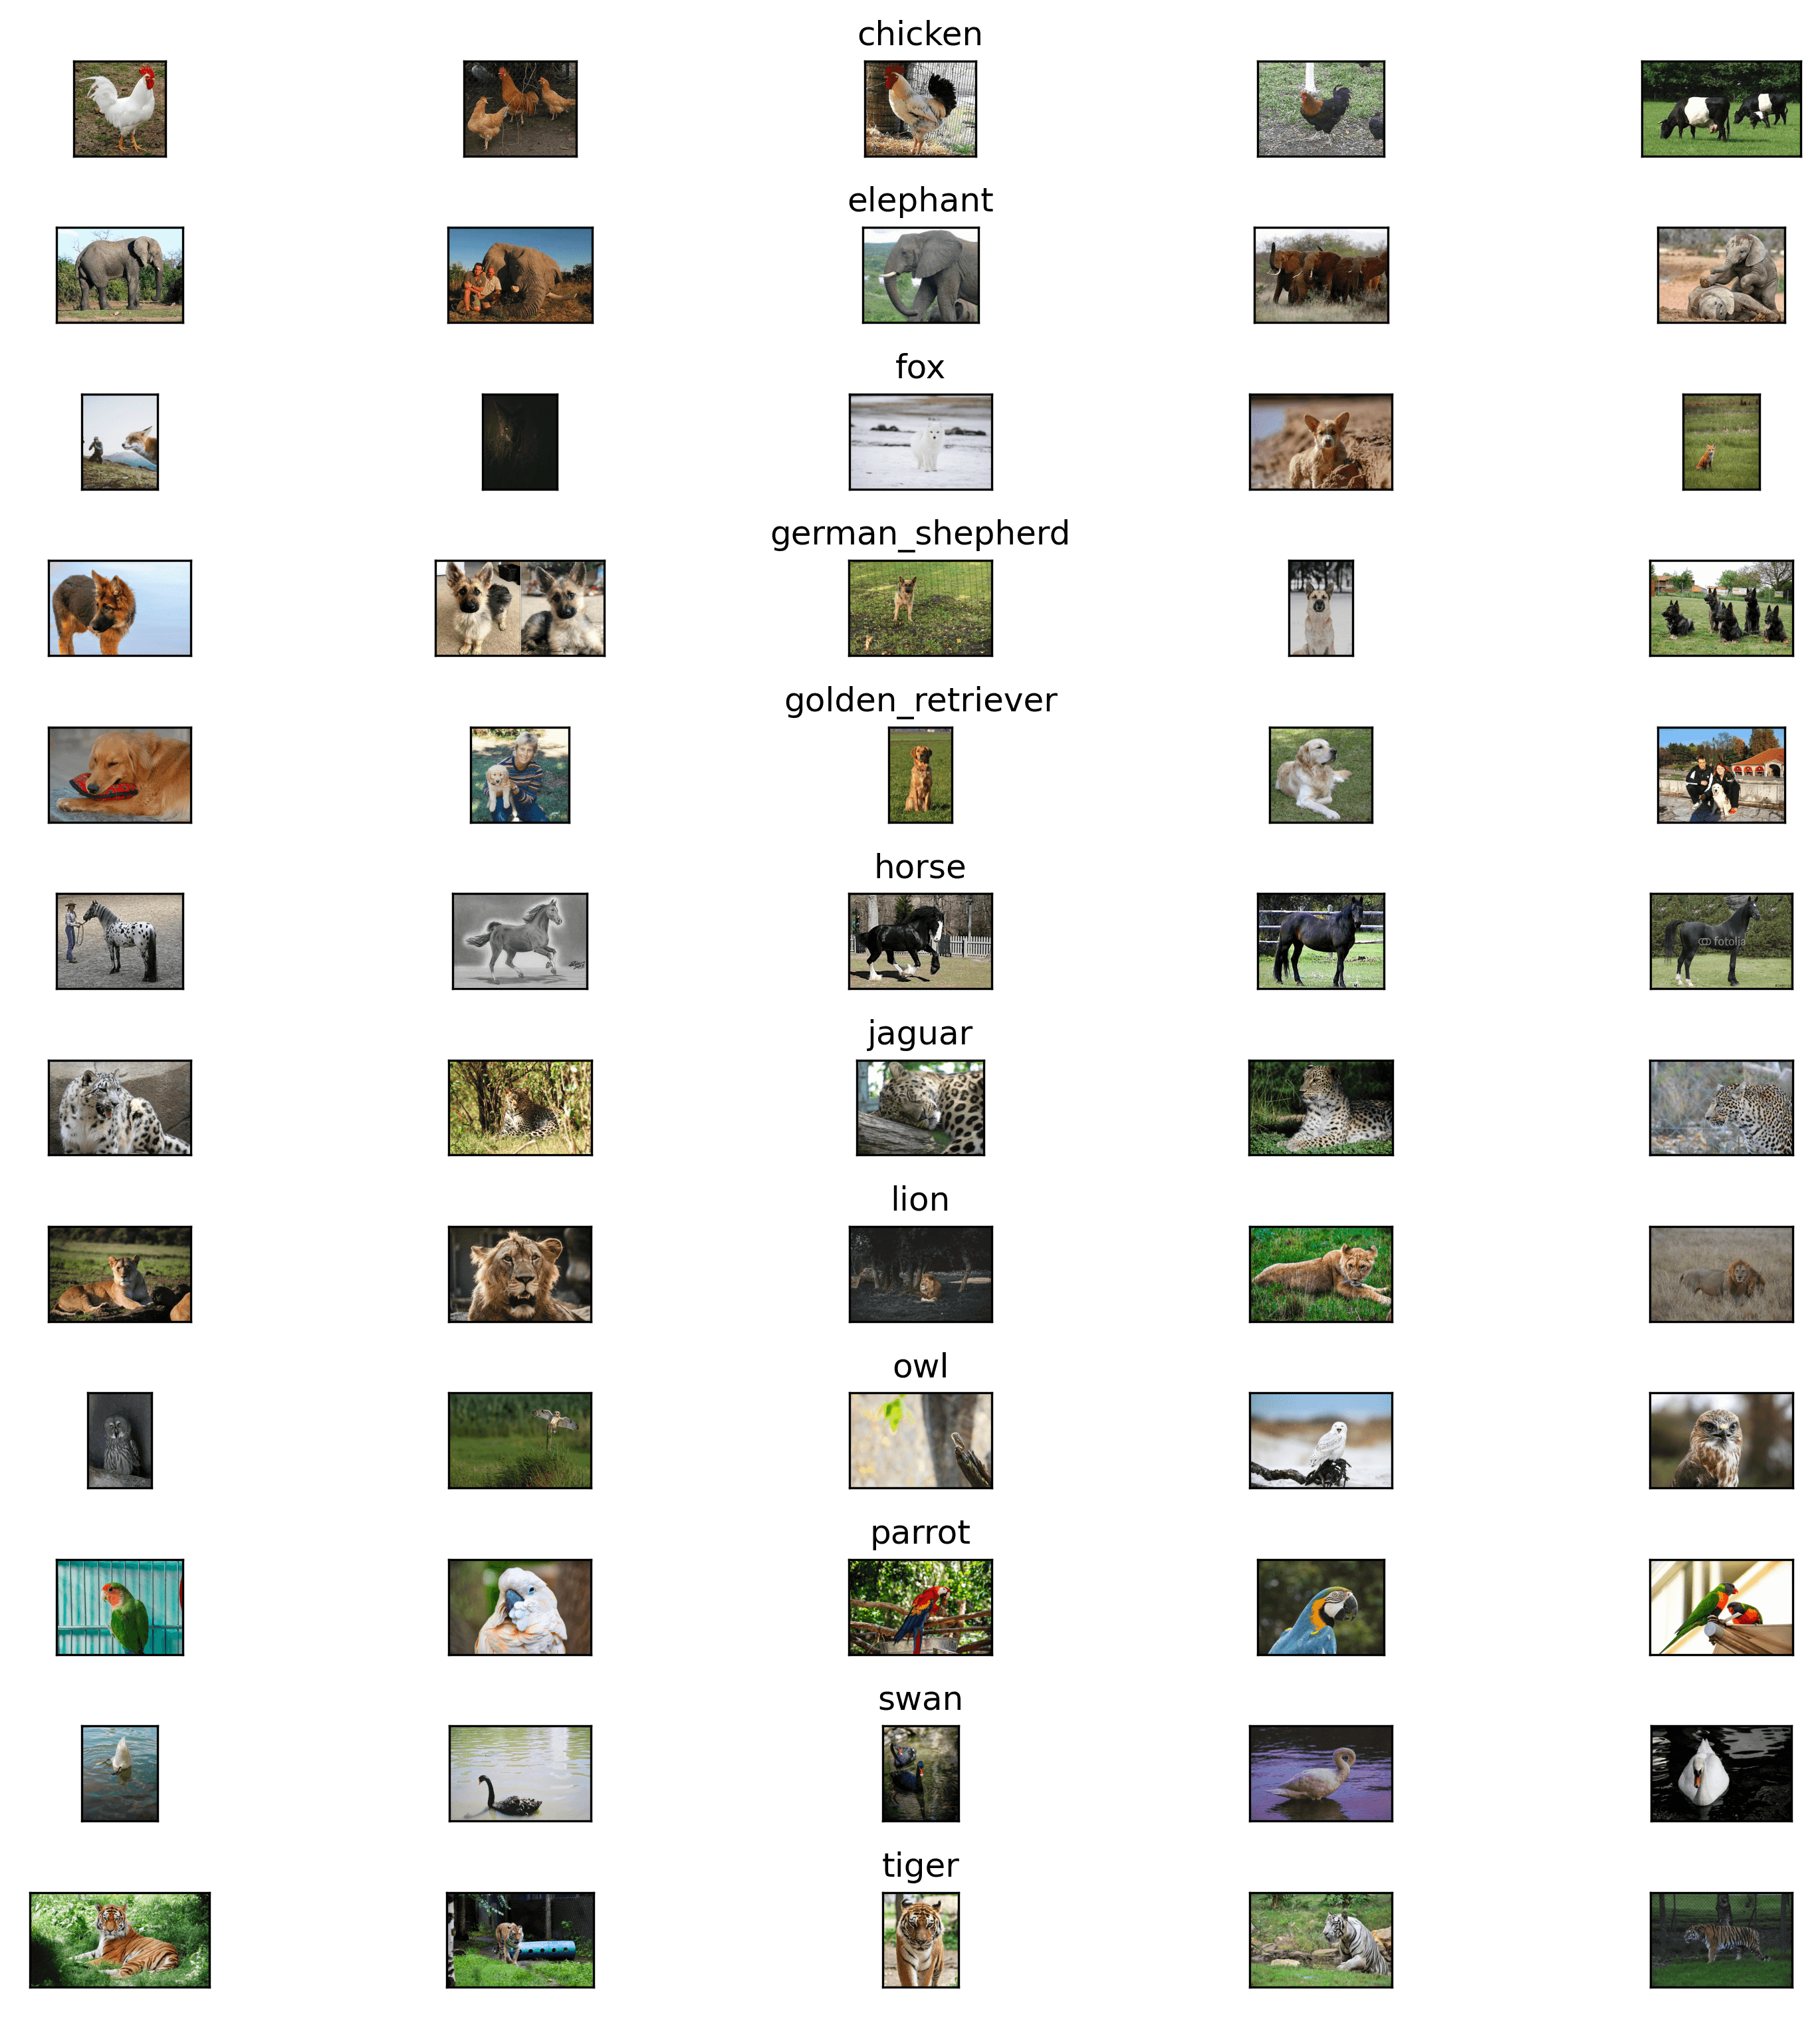
\includegraphics[width=0.70\linewidth]{images/1-data_analysis-labeled_data_overview.png}}
    \end{center}
    \captionsetup{width=0.65\linewidth}
    \captionsetup{justification=centering}
    \caption{An overview of the supplied data per class.}
    \label{fig:1-data_analysis-labeled_data_overview.png}
\end{figure}

%------------------------------------

\section*{Overview of features data}

\begin{figure}[H]
    \fbox{\includegraphics[width=1\linewidth]{images/1-data_analysis-feature_representation.png}}
    \captionsetup{width=0.85\linewidth}
    \captionsetup{justification=centering}
    \caption{An overview of the first 30 features data from a SIFT descriptor.}
    \label{fig:1-data_analysis-feature_representation}
\end{figure}

%------------------------------------

\section*{Linear baseline model - input optimisation (small)}

\begin{figure}[H]
  \centering
  \begin{minipage}[b]{0.4\textwidth}
    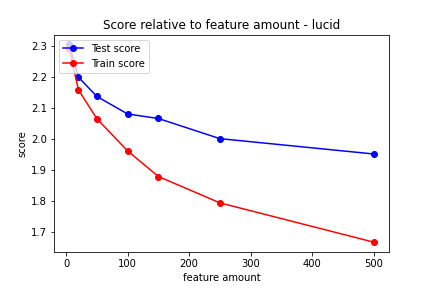
\includegraphics[width=\textwidth]{images/2-LBM-feature_amount_lucid_small_values.png}
  \end{minipage}
  \hfill
  \begin{minipage}[b]{0.4\textwidth}
    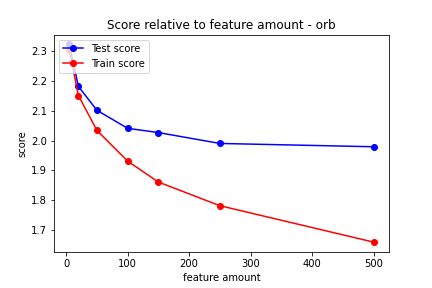
\includegraphics[width=\textwidth]{images/2-LBM-feature_amount_orb_small_values.png}
  \end{minipage}
\end{figure}

\begin{figure}[H]
  \centering
  \begin{minipage}[b]{0.4\textwidth}
    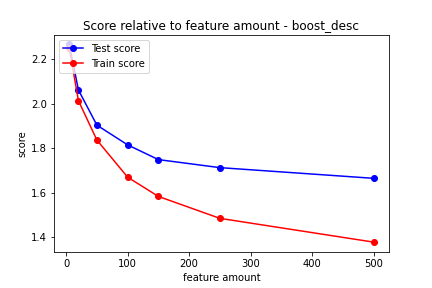
\includegraphics[width=\textwidth]{images/2-LBM-feature_amount_boost_desc_small_values.png}
  \end{minipage}
  \hfill
  \begin{minipage}[b]{0.4\textwidth}
    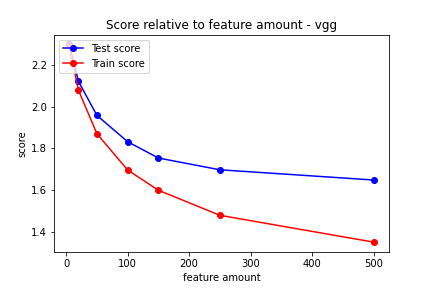
\includegraphics[width=\textwidth]{images/2-LBM-feature_amount_vgg_small_values.png}
  \end{minipage}
\end{figure}

\begin{figure}[H]
  \centering
  \begin{minipage}[b]{0.4\textwidth}
    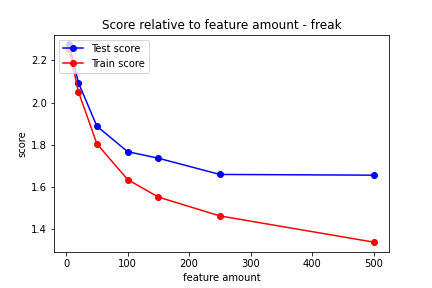
\includegraphics[width=\textwidth]{images/2-LBM-feature_amount_freak_small_values.png}
  \end{minipage}
  \hfill
  \begin{minipage}[b]{0.4\textwidth}
    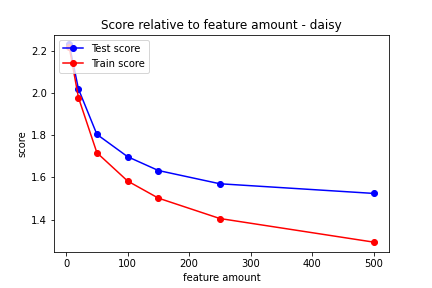
\includegraphics[width=\textwidth]{images/2-LBM-feature_amount_daisy_small_values.png}
  \end{minipage}
\end{figure}

\begin{figure}[H]
  \centering
  \begin{minipage}[b]{0.4\textwidth}
    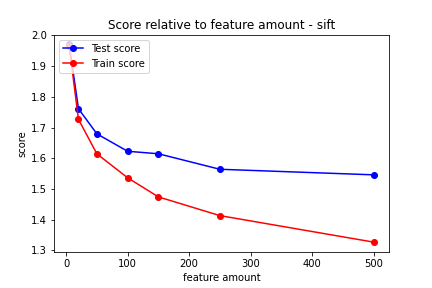
\includegraphics[width=\textwidth]{images/2-LBM-feature_amount_sift_small_values.png}
  \end{minipage}
\end{figure}

%------------------------------------

\section*{Linear baseline model - input optimisation (large)}

\begin{figure}[H]
  \centering
  \begin{minipage}[b]{0.4\textwidth}
    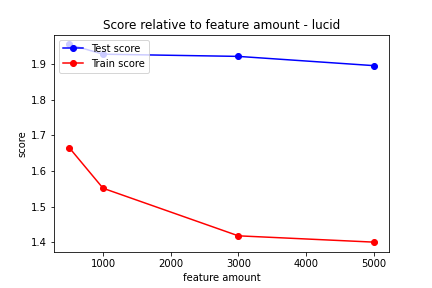
\includegraphics[width=\textwidth]{images/2-LBM-feature_amount_lucid_large_values.png}
  \end{minipage}
  \hfill
  \begin{minipage}[b]{0.4\textwidth}
    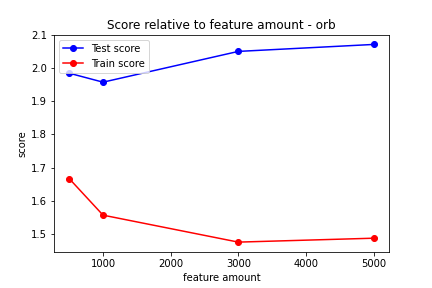
\includegraphics[width=\textwidth]{images/2-LBM-feature_amount_orb_large_values.png}
  \end{minipage}
\end{figure}

\begin{figure}[H]
  \centering
  \begin{minipage}[b]{0.4\textwidth}
    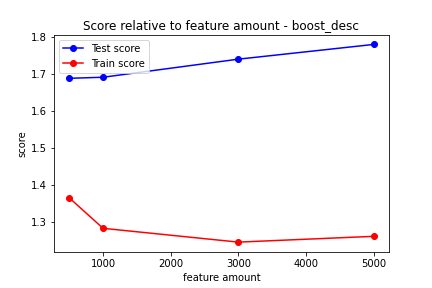
\includegraphics[width=\textwidth]{images/2-LBM-feature_amount_boost_desc_large_values.png}
  \end{minipage}
  \hfill
  \begin{minipage}[b]{0.4\textwidth}
    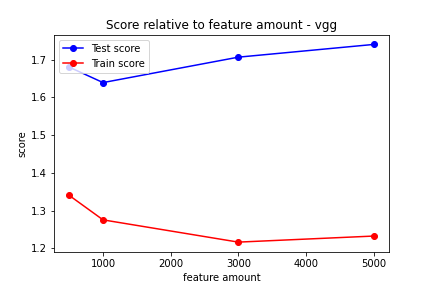
\includegraphics[width=\textwidth]{images/2-LBM-feature_amount_vgg_large_values.png}
  \end{minipage}
\end{figure}

\begin{figure}[H]
  \centering
  \begin{minipage}[b]{0.4\textwidth}
    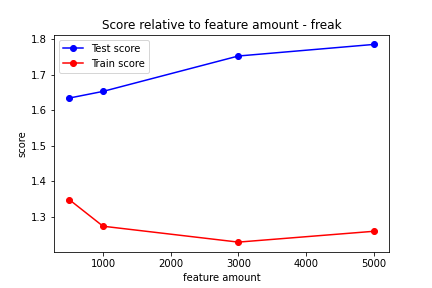
\includegraphics[width=\textwidth]{images/2-LBM-feature_amount_freak_large_values.png}
  \end{minipage}
  \hfill
  \begin{minipage}[b]{0.4\textwidth}
    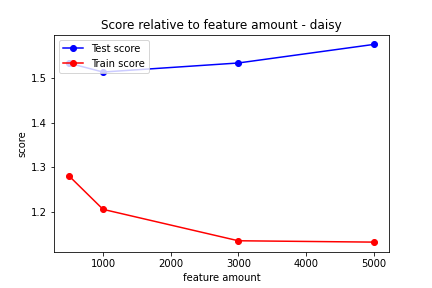
\includegraphics[width=\textwidth]{images/2-LBM-feature_amount_daisy_large_values.png}
  \end{minipage}
\end{figure}

\begin{figure}[H]
  \centering
  \begin{minipage}[b]{0.4\textwidth}
    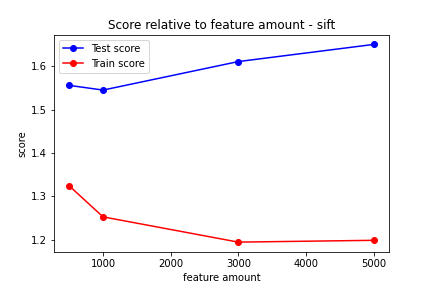
\includegraphics[width=\textwidth]{images/2-LBM-feature_amount_sift_large_values.png}
  \end{minipage}
\end{figure}

%------------------------------------

\section*{Linear baseline model - optimal DAISY}

\begin{figure}[H]
    \fbox{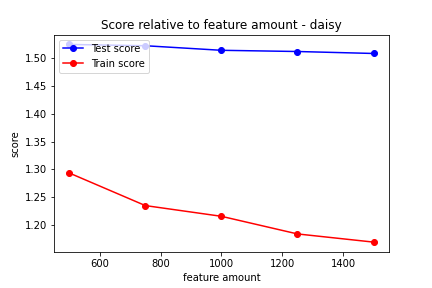
\includegraphics[width=1\linewidth]{images/2-LBM-feature_amount_daisy_daisy_optimal.png}}
    \captionsetup{width=0.85\linewidth}
    \captionsetup{justification=centering}
    \caption{An extra test for finding the optimal feature amounts for the DAISY descriptor.}
    \label{fig:2-LBM-feature_amount_daisy_daisy_optimal}
\end{figure}

%------------------------------------

\section*{Linear baseline model - class weight parameter}

\begin{figure}[H]
    \fbox{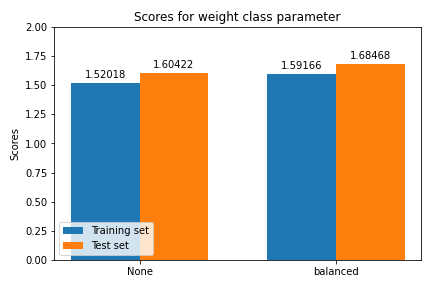
\includegraphics[width=1\linewidth]{images/2-LBM-model_weight_class.png}}
    \captionsetup{width=0.85\linewidth}
    \captionsetup{justification=centering}
    \caption{Average multi-class Log Loss score over 10 iterations.}
    \label{fig:2-LBM-model_weight_class}
\end{figure}

%------------------------------------

\section*{Linear baseline model - fit intercept parameter}

\begin{figure}[H]
    \fbox{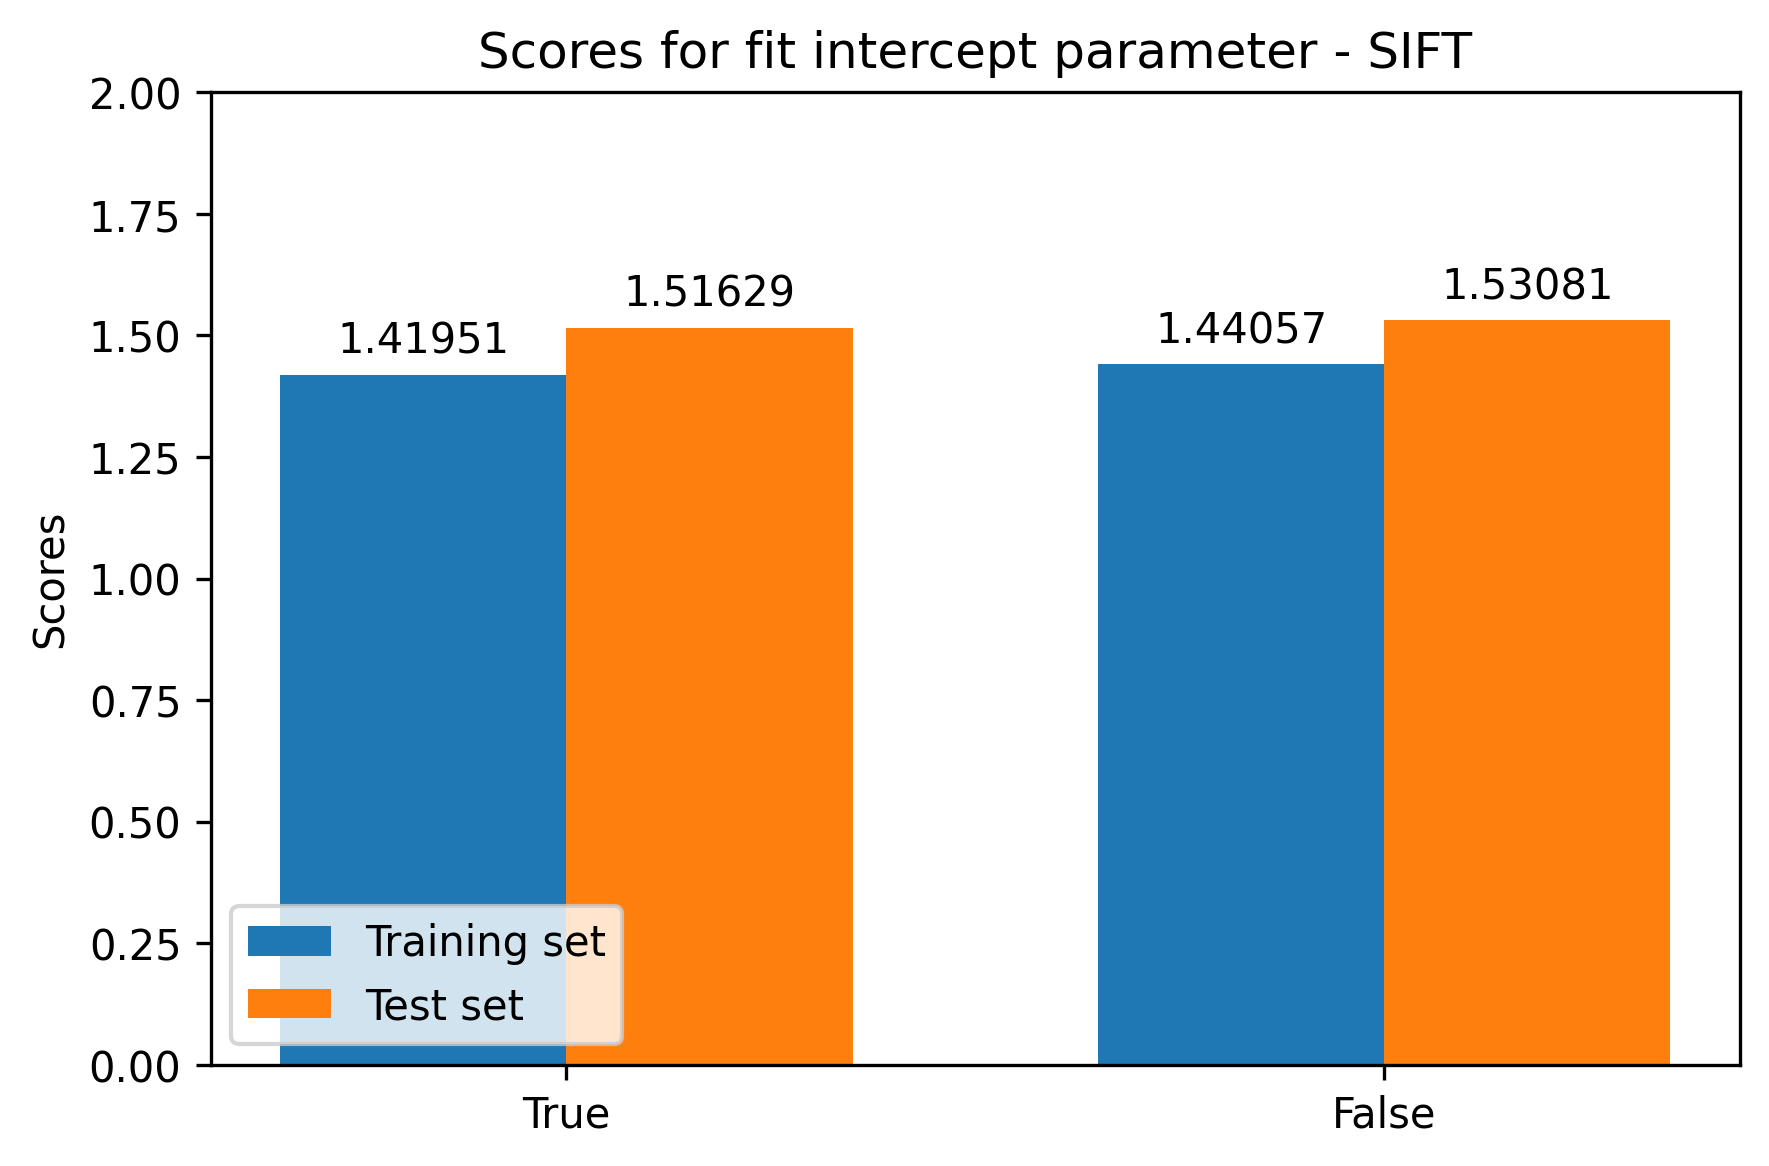
\includegraphics[width=1\linewidth]{images/2-LBM-model_fit_intercept.png}}
    \captionsetup{width=0.85\linewidth}
    \captionsetup{justification=centering}
    \caption{Average multi-class Log Loss score over 5 iterations.}
    \label{fig:2-LBM-model_fit_intercept}
\end{figure}

%references list
\nocite{*}
\printbibliography[heading=bibintoc, title={References}]

%START appendix
\chapter*{Appendix A: Working and representation of the descriptors}
\addcontentsline{toc}{chapter}{Appendix A: Working and representation of the descriptors}

\section*{Feature extraction}

Some feature extraction has already been provided.
In short, images are converted from there typical RGB representation to a numerical representation of interesting points, which can be used as input for our model.
How this is done and could be optimized is briefly discussed here since it consists of provided code for the Kaggle competition.

Instead of using the whole image as data, only a select few of \textit{interesting points} of the image are taken into consideration.
These interesting points of an image are often found by using the \emph{Shi-Tomasi corner detector}, but some descriptors have different implementations.
As the name suggests, these interesting points are \textit{strong corners on an image}.

Shown in figure \ref{fig:1-poi} is an example output of interesting points found by the Shi-Tomasi corner detector.
It's clear that its performance varies a lot, but finding interesting points isn't an easy task and thus the results are better then they might seem on first sight.
It's also noted that SIFT is used for the models in this report, which uses a different, patented, technique for interesting point detection.

\begin{figure*}[ht]
    \centering
    \begin{subfigure}{.35\textwidth}
        \centering
        \fbox{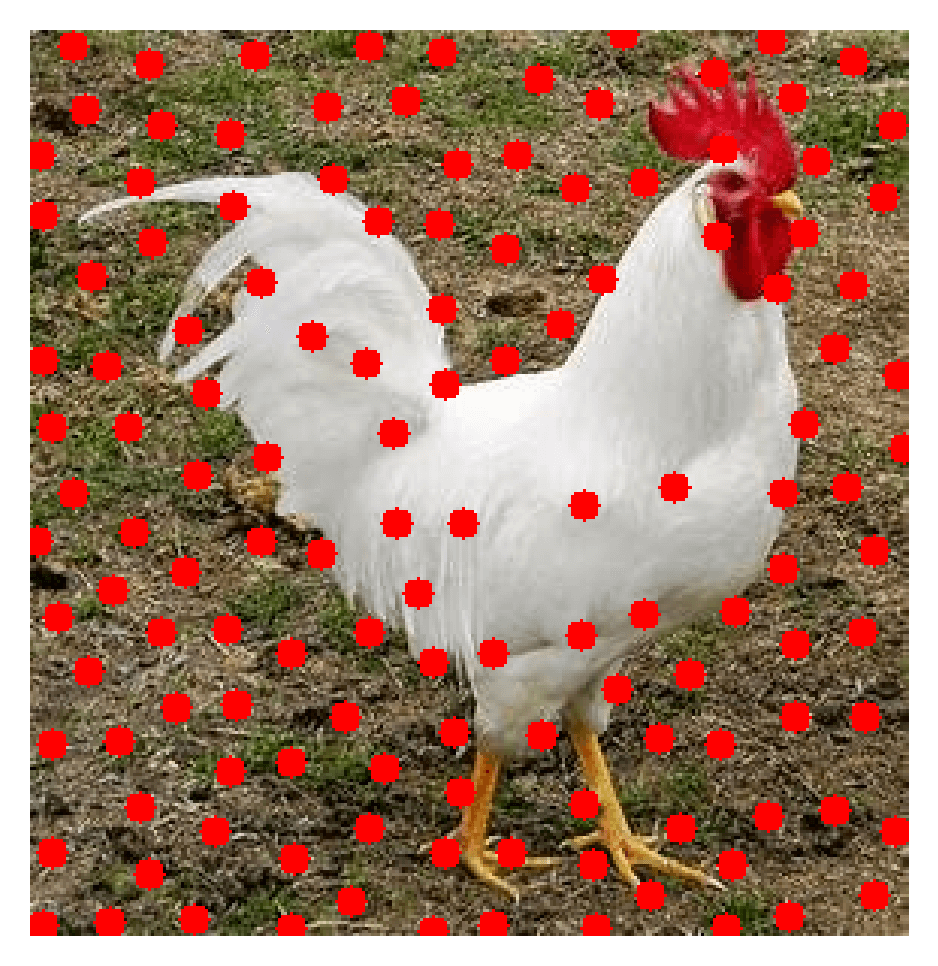
\includegraphics[width=0.9\textwidth]{images/1/1-data_analysis-POI_chicken.png}}
        \captionsetup{width=0.9\linewidth}
        \captionsetup{justification=centering}
        \caption{First chicken in data.}
    \end{subfigure}
    \hspace{1cm}
    \begin{subfigure}{.52\textwidth}
        \centering
        \fbox{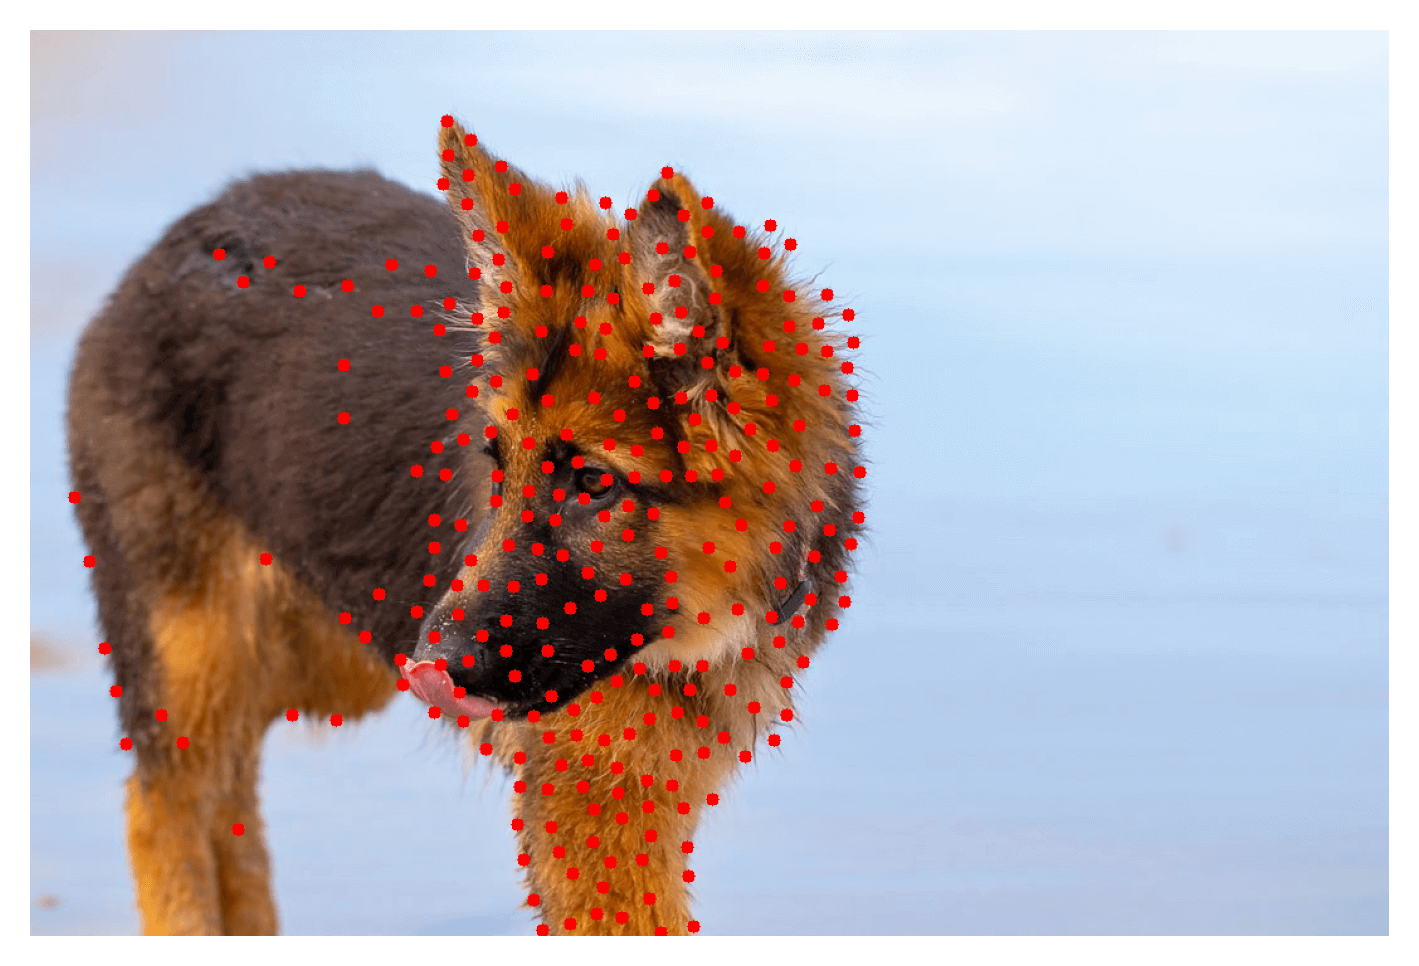
\includegraphics[width=0.9\textwidth]{images/1/1-data_analysis-POI_german_shepherd.png}}
        \captionsetup{width=0.9\linewidth}
        \captionsetup{justification=centering}
        \caption{First German shepherd in train data}
    \end{subfigure}
    \captionsetup{width=0.8\linewidth}
    \captionsetup{justification=centering}
    \caption{Points of interest found by the Shi-Tomasi corner detector.}
    \label{fig:1-poi}
\end{figure*}


%------------------------------------

\section*{The numerical representation}

These interesting points now need to be represented by numerical values that have actual meaning.
Remember from section \ref{section:DA_deeper_look_data} that the provided images differ a lot.
Thus the numerical representation, generated by a descriptor, has to be so that it minifies the impact of different lighting, scaling...
afterwards, these values can be clustered together using the \texttt{createCodebook} function which uses Mini-Batch K-Means clustering.
This could also benefit from fine-tuning.

An overview showing histograms for each word (cluster) and a corresponding correlation matrix when opting for SIFT with 30 clusters is shown in figure \ref{fig:1-cm}.
It is visible that the values are normalized.
This would have to be checked for all descriptors used and perhaps some outliers would need to be removed.
The correlation between these clusters doesn't seem too dramatic in this case ($|$correlation value$| \neq 1 $).
A low correlation between clusters is mostly positive for model building since it suggests each cluster represent a distinct concept.
This is again something that would have to be checked for different parameters.

\begin{figure}[H]
    \centering
    \begin{subfigure}{.45\textwidth}
        \centering
        \fbox{\includegraphics[width=0.7\textwidth]{images/1/1-data_analysis-feature_representation.png}}
        \captionsetup{width=0.9\linewidth}
        \captionsetup{justification=centering}
        \caption{Histogram for each cluster.}
    \end{subfigure}
    \hspace{1cm}
    \begin{subfigure}{.45\textwidth}
        \centering
        \fbox{\includegraphics[width=0.8\textwidth]{images/1/1-data_analysis-correlation_matrix.png}}
        \captionsetup{width=0.9\linewidth}
        \captionsetup{justification=centering}
        \caption{Correlation matrix for all clusters.}
    \end{subfigure}
    \captionsetup{width=0.8\linewidth}
    \captionsetup{justification=centering}
    \caption{Data analysis of encoded images using SIFT with 30 clusters.}
    \label{fig:1-cm}
\end{figure}


%------------------------------------------------------------------------------------------------------------------------------------------------


\chapter*{Appendix B: Important LBM parameters}
\addcontentsline{toc}{chapter}{Appendix B: Important LBM parameters}

As found in the documentation of the \texttt{LogisticRegression} function available in the SciKit Learn library there are multiple (optional) parameters \citep{scikit_learn}.
The most interesting ones are:

\begin{itemize}
    \item \emph{solver}
    \begin{itemize}
        \item Specifies which solver should be used for the optimization problem in the model.
        \item \emph{lbfgs} is used as default and whilst a little slow, this parameter doesn't require further fine-tuning.
    \end{itemize}
    \item \emph{penalty}
    \begin{itemize}
        \item Since the \emph{lbfgs} solver is used, the default \emph{l2} penalization norm is the only one that can be used.
    \end{itemize}
    \item \emph{class\_weight}
    \begin{itemize}
        \item This parameter defaults to None but can be set to balanced to take into account the unbalance in our data, as discussed in section \ref{section:DA_data_distribution}.
        \item The results with this parameter set to balanced will be studied.
    \end{itemize}
    \item \emph{C}
    \begin{itemize}
        \item The regularisation hyperparameter C defaults to 1. Fine-tuning this could boost performance.
    \end{itemize}
    \item \emph{max\_iter}
    \begin{itemize}
        \item This parameter can be changed so that convergence might be found, which is not the case right now.
    \end{itemize}
    \item \emph{fit\_intercept}
    \begin{itemize}
        \item Boolean that specifies if a constant (a.k.a. bias or intercept) should be added to the decision function.
        \item The results with this parameter set to true and false should be checked.
    \end{itemize}
\end{itemize}

%------------------------------------------------------------------------------------------------------------------------------------------------

\end{document}
